\clearpage
\subsectionold{\olly}
\myindex{\olly}

Компилируем этот пример в MSVC 2010 с ключами \TT{/GS- /MD} и запускаем в \olly.
Открываем окна данных и стека по адресу, который передается в качестве первого аргумента в функцию \TT{GetSystemTime()}, 
ждем пока эта функция исполнится, и видим следующее:

\begin{figure}[H]
\centering
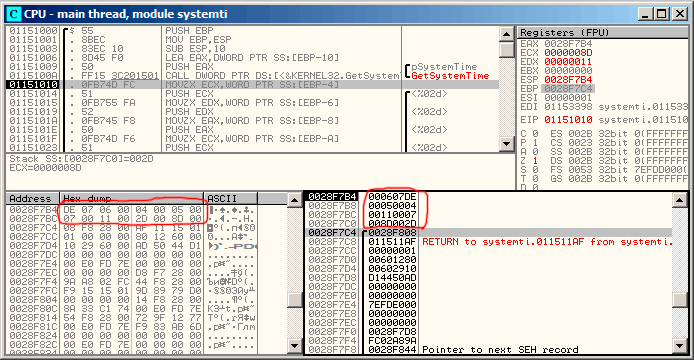
\includegraphics[scale=\FigScale]{patterns/15_structs/1_systemtime/olly_systemtime1.png}
\caption{\olly: \TT{GetSystemTime()} только что исполнилась}
\label{fig:struct_olly_1}
\end{figure}

Точное системное время на моем компьютере, в которое исполнилась функция, это 9 декабря 2014, 22:29:52:

\begin{figure}[H]
\centering
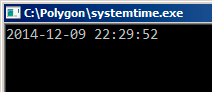
\includegraphics[scale=\NormalScale]{patterns/15_structs/1_systemtime/olly_systemtime2.png}
\caption{\olly: Вывод \printf}
\label{fig:struct_olly_2}
\end{figure}

Таким образом, в окне данных мы видим следующие 16 байт: 
\begin{lstlisting}
DE 07 0C 00 02 00 09 00 16 00 1D 00 34 00 D4 03
\end{lstlisting}

Каждые два байта отражают одно поле структуры. 
А так как порядок байт (\gls{endianness}) \IT{little endian},
то в начале следует младший байт, затем старший.
Следовательно, вот какие 16-битные числа сейчас записаны в памяти:

\begin{center}
\begin{tabular}{ | l | l | l | }
\hline
\headercolor{} Шестнадцатеричное число & 
\headercolor{} десятичное число & 
\headercolor{} имя поля \\
\hline
0x07DE & 2014	& wYear \\
\hline
0x000C & 12	& wMonth \\
\hline
0x0002 & 2	& wDayOfWeek \\
\hline
0x0009 & 9	& wDay \\
\hline
0x0016 & 22	& wHour \\
\hline
0x001D & 29	& wMinute \\
\hline
0x0034 & 52	& wSecond \\
\hline	
0x03D4 & 980	& wMilliseconds \\
\hline
\end{tabular}
\end{center}

В окне стека, видны те же значения, только они сгруппированы как 32-битные значения.

Затем \printf просто берет нужные значения и выводит их на консоль.

Некоторые поля \printf не выводит (\TT{wDayOfWeek} и
\TT{wMilliseconds}), но они находятся в памяти и доступны для использования.

